\chapter{Signal d'entrée et réglage de volume}

\begin{center}
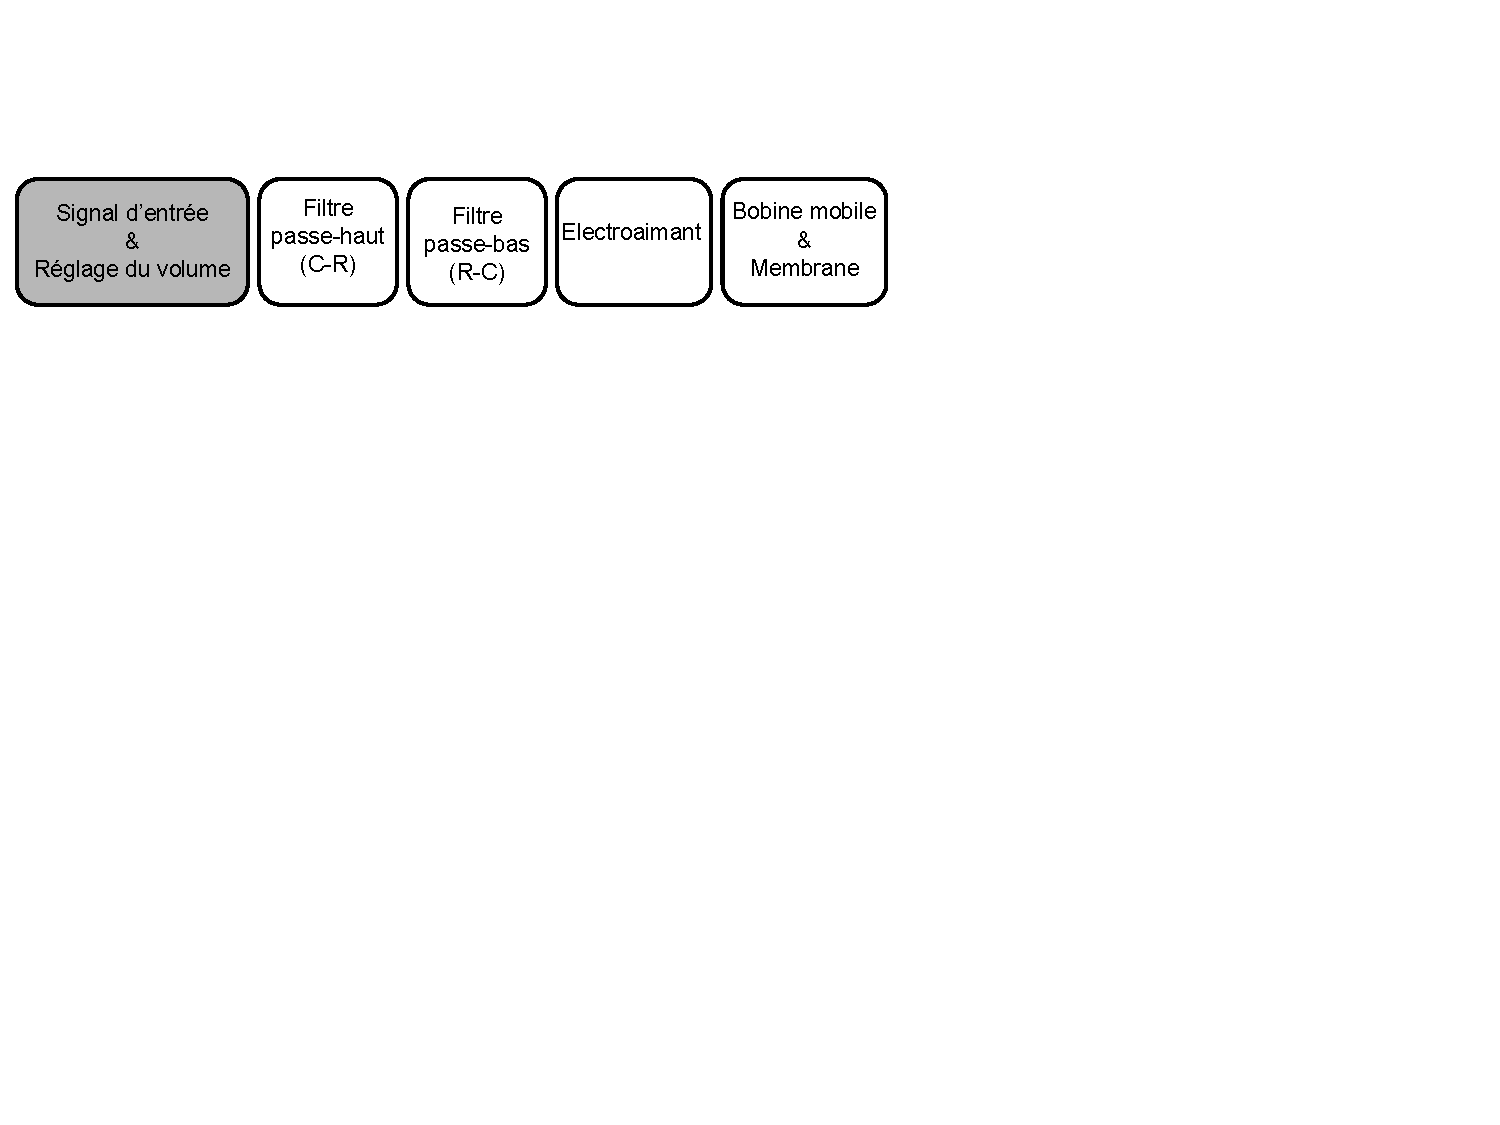
\includegraphics[width=\textwidth]{img/Schemabloc1}
\end{center}

\section{Introduction}
La sortie typique d'un smartphone à plein volume est une différence de potentiel de $\milli\volt$ . Cela peut paraitre peu, 
mais une telle amplitude peut être dangereuse pour les puces électroniques du circuit si elle n'est pas diminuée par
un dispositif quelconque. De plus, pouvoir faire varier l'amplitude permet de faire varier le volume de manière
indépendante par rapport au smartphone.
\section{Résolution}
Pour répondre à ces deux attentes, il nous suffit de réaliser un diviseur de tension réglable, que nous avons réalisé 
à l'aide d'un potentiomètre à l'entrée de la plaquette électronique. Le schéma ci dessous illustre la situation. Le potentiomètre 
à été schématisé en 2 résistances simples.\\

\begin{figure}	
\begin{center}
\begin{circuitikz} \draw
 (1,2)
  to[R,v=$v_1$, l=$R_1$, *-*] (1,0)
 (1,2) to[short, *-o] (0,2)
  node[anchor=east]{A}
 (1,0) to [R,v=$v_2$, l=$R_2$] (1,-2)
 (1,0) to[short, *-o] (3,0)
node[anchor=west]{B}
 (1,-2)node[ground]{}
;\end{circuitikz}
\end{center}
\caption{Potentiomètre}		
\label{potentiometre}		
\end{figure}

La différence de tension $V =  v_1 + v_2$ est la différence de potentiel provenant du smartphone. 
En utilisant la loi d'ohm, nous obtenons $V = I (R_1 + R_2)$ et $v_2 = I R_2$. Puisque $I = \frac{V}{R_1+R_2}$, nous obtenons 
$v_2 = \frac{V R_2}{R_1+R_2}$. $R_1+R_2$ est la résistance totale du potentiomètre, $R_1$ et $R_2$ sont inversément proportionnelles. Plus $R_2$ 
sera grande et donc proche de la résistance totale du potentiomètre, plus la tension en $B$ sera proche de la tension fournie en $A$. Nous voyons 
donc bien qu'en faisant varier le sélecteur du potentiomètre, nous faisons varier la tension en $B$, ce qui fera varier le volume du 
haut-parleur.